\pagebreak
\section{Meta Model}\label{metamodel}
The classes in the Ecore meta-model are described in this section along
with the OCLinEcore validation steps that are applied.

For reference, the full meta-model is displayed first and the individual
components after.
\begin{figure}[h]
\centering
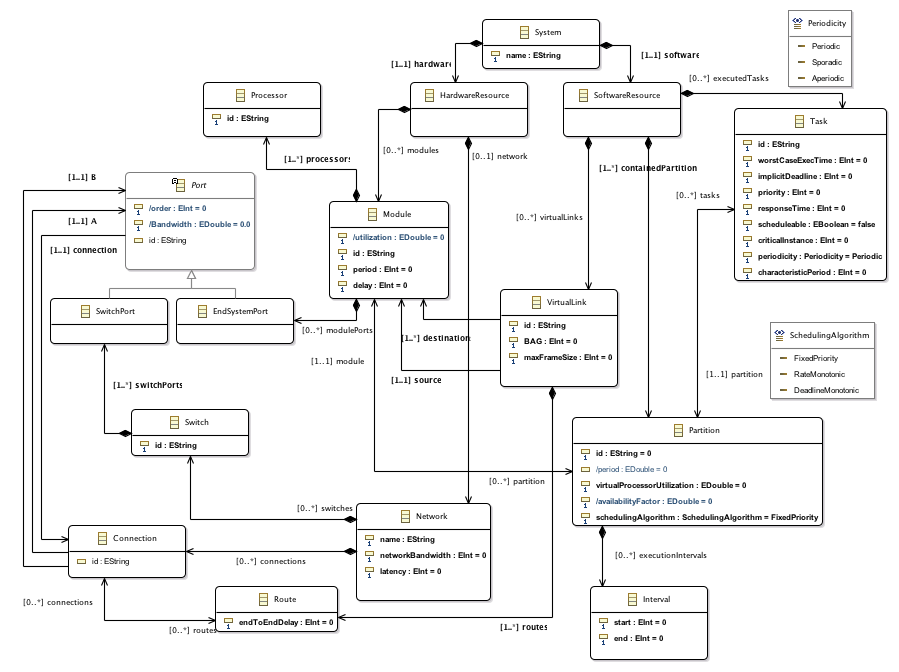
\includegraphics[width=0.8\textwidth]{metamodel_full.png}
\caption{Full UML meta-model}
\label{fig:fullmodel} % adding labels for references
\end{figure}

% Now all of the model elements
\paragraph{System}
The root object for an instance of the meta model. This class
serves to hierarchically organize the rest of the classes.
\begin{lstlisting}[caption=System constraints]
class System {
    property hardware : HardwareResource { composes };
    attribute name : String;
    property software : SoftwareResource { composes };
}
\end{lstlisting}

\paragraph{Hardware and Software Resources}
These two classes hierarchically organize other model elements.
\begin{lstlisting}[caption=Hardware and Software constraints]
class SoftwareResource {
    property executedTasks : Task[*] { ordered composes  };
    property containedPartitions : Partition[+] { ordered composes  };
    property virtualLinks : VirtualLink[*] { ordered composes  };
}
class HardwareResource {
    property modules : Module[*] { ordered composes  };
    property network : Network[?] { composes  };
}
\end{lstlisting}

\paragraph{Task}
A task is a software service that has well defined temporal activation parameters.
\begin{lstlisting}[caption=Task constraints]
class Task {
    attribute id : String { id  };
    attribute worstCaseExecTime : ecore::EInt = '0';
    attribute implicitDeadline : ecore::EInt;
    attribute priority : ecore::EInt;
    attribute responseTime : ecore::EInt;
    attribute scheduleable : Boolean;
    attribute criticalInstance : ecore::EInt;
    attribute periodicity : Periodicity = 'Periodic';
    attribute characteristicPeriod : ecore::EInt;
    property partition#tasks : Partition;
    invariant PositiveWCET: worstCaseExecTime > 0;
    invariant ExecutionAndDeadlineAllowsCompletion:
	worstCaseExecTime <= implicitDeadline;
    invariant ExecutionAndPeriodAllowsCompletion: 
	if (periodicity <> Periodicity::Aperiodic)
	    then worstCaseExecTime <= characteristicPeriod
	else true
	    endif;
    invariant DeadlineLessThanPeriod: implicitDeadline <= characteristicPeriod;
    invariant PositivePeriod: characteristicPeriod > 0;
}
\end{lstlisting}
\paragraph{Constraint Details} 
\begin{description}
\item[\texttt{ExecutionAndDeadlineAllowsCompletion}] The WCET must be less than or equal to the implicit deadline otherwise the task will never complete in time.
\item[\texttt{ExecutionAndPeriodAllowsCompletion}] The WCET must be less than or equal to the period of the task. This is only a constraint on tasks that are not 
\textit{aperiodic} tasks: tasks without a minimum time between arrivals.
\item[\texttt{DeadlineLessThanPeriod}] The deadline of the task must be less than or equal to the period otherwise multiple instances of the task will exist simultaneously.
\end{description}
\paragraph{Partition}
A partition is a list of time intervals and a period. Tasks are assigned to partitions.
\begin{lstlisting}[caption=Partition constraints]
class Partition {
    attribute id : String = '0' { id  };
    attribute period : ecore::EDouble[?] = '0' { derived readonly  } {
derivation:
	if (module->oclIsInvalid() or module->oclIsUndefined() or module = null)
	    then 0.0
	else self.module.period
	    endif;
    }
    property executionIntervals : Interval[*] { ordered composes  };
    attribute virtualProcessorUtilization : ecore::EDouble = '0';
    attribute availabilityFactor : ecore::EDouble = '0' { derived  } { derivation:
	--check for divide by zero!
	    if (period <> 0)
		then executionIntervals->
		    collect(i : Interval | i.end - i.start)->sum() / period
	    else 0.0
		endif;
    }
    attribute schedulingAlgorithm : SchedulingAlgorithm;
    property tasks#partition : Task[*] { ordered  };
    property module#partition : Module;
    invariant PositivePeriod: period > 0;
    invariant AvailibilityFactorLessThanOrEqualToOne: availabilityFactor <= 1;
    invariant PeriodSpansIntervals:
	let sortedIntervals : Sequence(Interval) = executionIntervals->
	sortedBy(start) in
	if (sortedIntervals->size() > 1)
	    then sortedIntervals->last().end <= period
	else true
	    endif;
    invariant NonOverlappingIntervals:
	if (executionIntervals->size() <= 1)
	    then true -- Nothing can overlap if there is only one or none!
	else
	    let sortedIntervals : Sequence(Interval) = executionIntervals->
		sortedBy(i : Interval | i.start) in
		sortedIntervals->
		subSequence(1, sortedIntervals->size() - 1)->
		forAll(i : Interval |
			i.end <= sortedIntervals->at(1 + sortedIntervals->indexOf(i)).start)
		endif;
}
\end{lstlisting}
\paragraph{Constraint Details}
\begin{description}
\item[\texttt{period}] The period of a Task is defined to be the period of the module it executes on.
This simplifies validating that no partitions overlap within a module.
\item[\texttt{availabilityFactor}] The fraction of time this partition occupies within a module. This
is not the same as the virtual processor utilization which is the fraction of time that any task
is executing in a partition.
\item[\texttt{PeriodSpansIntervals}] The intervals defined in a partition must be wholly contained
within $t = (0,T)$. 
\item[\texttt{NonOverlappingIntervals}] No two intervals within a partition may overlap. This is
acchieved by imposing an ordering on the intervals and checking to make sure that
no two sequential intervals overlap.
\end{description}
\paragraph{Interval}
An interval is a period of execution for tasks in a partition.
\begin{lstlisting}[caption=Interval constraints]
class Interval {
    attribute start : ecore::EInt;
    attribute end : ecore::EInt;
    invariant EndAfterStart: end >= start;
    invariant NonZeroLength: end <> start;
}
\end{lstlisting}
\subsection{Complex Validation}
Some validation could not be expressed in \texttt{OCLinEcore}.
\paragraph{Network Invariants} There are invariants for a \texttt{VirtualLink}
that are better expressed through graph algorithms.
\begin{lstlisting}[caption=VirtualLink graph invariants]
    invariant PathExists;
    invariant RoutesConnectSourceToDestinations;
    invariant NoCycles;
\end{lstlisting}
These invariants are expressed in the \texttt{fr.ensma.realtimescheduling.util.RealtimeschedulingValidator.java}
class as part of the validation code.
We used the free and open source Java graph library \href{http://jgrapht.org/}{\textbf{JGraphT}}.
The first constraint \texttt{PathExists} verifies that there is atleast one path possible
between the source of a virtual link and each of its destinations. We consider all
of the ports in the network as nodes and all of the ports of a switch are fully connected.
Regular connections are edges.
First we build the graph.
\begin{minted}[
frame=lines,
    framesep=2mm,
    baselinestretch=1.2,
    fontsize=\footnotesize,
    linenos
    ]{java}
    private void buildGraph(fr.ensma.realtimescheduling.System system) {
	networkGraph = new SimpleGraph<>(DefaultEdge.class); 
	for (Switch switch_ : system.getHardware().getNetwork().getSwitches()) { 
	    for (Port port : switch_.getSwitchPorts()) 
		networkGraph.addVertex(port);
	    for (Port port : switch_.getSwitchPorts()) 
		for (Port port2 : switch_.getSwitchPorts()) 
		    // within a switch, all ports are "connected" to each other.
		    if (port2 != port) 
			networkGraph.addEdge(port, port2);
	}
	for (Module module : system.getHardware().getModules()) 
	    for (Port port : module.getModulePorts()) 
		networkGraph.addVertex(port);
	for (Connection connection : system.getHardware().getNetwork()
		.getConnections()) 
	    if (connection.getA() != null && connection.getB() != null) 
		networkGraph.addEdge(connection.getA(), connection.getB());
    }
\end{minted}
Then we ask JGraphT to check the connectivity of every virtual link.
\begin{minted}[
    frame=lines,
    framesep=2mm,
    baselinestretch=1.2,
    fontsize=\footnotesize,
    linenos
    ]{java}
    ConnectivityInspector<Port, DefaultEdge> inspector = new ConnectivityInspector<>(networkGraph);
    boolean pathExists = false;
    try {
all: for (Port sourcePort : virtualLink.getSource().getModulePorts()) 
	 for (Module destination : virtualLink.getDestinations()) 
	     for (Port destinationPort : destination.getModulePorts()) {
		 pathExists = inspector.pathExists(sourcePort,destinationPort);
		 if (!pathExists)
		     break all;
	     }
    } catch (Exception e) {
	e.printStackTrace();
    }
\end{minted}
The next constraint verifies that the specified routes actually connect the correct modules.
This is done by `walking' a route and verifying that the last connection
connects one of the destinations. If, at the end, all destinations have been reached,
then all of the routes connect all of the destinations and the virtual link is valid.
\begin{minted}[
    frame=lines,
    framesep=2mm,
    baselinestretch=1.2,
    fontsize=\footnotesize,
    linenos
]{java}
boolean success = false;
List<Module> destinationsHit = new ArrayList<>();
destinationsHit.addAll(virtualLink.getDestinations());
try {
    for (Route r : virtualLink.getRoutes()) {
	Port first = virtualLink.getSource().getModulePorts().stream()
	    .filter(esp -> r.getConnections()
		.contains(esp.getConnection()))
	    .findFirst()
	    .get();
	Port current = first;
	List<Connection> allConnections = new ArrayList<>();
	allConnections.addAll(r.getConnections());
	while (allConnections.size() != 1) {
	    allConnections.remove(current.getConnection());
	    current = Flow.getOpposite(current);
	    current = ((Switch) (current.eContainer())).getSwitchPorts().stream()
		.filter(sp -> allConnections.contains(sp.getConnection()))
		.findFirst()
		.orElseThrow(() -> new Exception());
	}
	// success if any of the destination ports are one of the two
	// ports
	// of the remaining connection of routes
	success = virtualLink.getDestinations().stream()
	    .anyMatch(module -> {
		    boolean matches = module.getModulePorts().contains(allConnections.get(0).getB());
		    destinationsHit.remove(module);
		    return matches;
		    })
	|| /* OR */
	    virtualLink.getDestinations().stream()
	    .anyMatch(module -> {
		    boolean matches = module.getModulePorts().contains(allConnections.get(0).getA());
		    destinationsHit.remove(module);
		    return matches;
		    });

    }
} catch (Exception e) {
    e.printStackTrace();
    success = false;
}
\end{minted}
The cycle checker is not implemented. See section \ref{future}.
